%% LyX 2.1.4 created this file.  For more info, see http://www.lyx.org/.
%% Do not edit unless you really know what you are doing.
\documentclass[a4paper,oneside,brazil,11pt,a4paper,openright,titlepage,usenames,dvipsnames]{book}
\usepackage[utf8]{inputenc}
\usepackage[T1]{fontenc}
\usepackage[brazilian]{babel}
\usepackage{lmodern}
%\usepackage{times}
\setcounter{secnumdepth}{3}
\setcounter{tocdepth}{3}
\usepackage{array}
\usepackage{verbatim}
\usepackage{calc}
\usepackage{textcomp}
\usepackage{amssymb}
\usepackage[pdf]{graphviz}

\makeatletter

%%%%%%%%%%%%%%%%%%%%%%%%%%%%%% LyX specific LaTeX commands.
\pdfpageheight\paperheight
\pdfpagewidth\paperwidth

%% Because html converters don't know tabularnewline
\providecommand{\tabularnewline}{\\}

%%%%%%%%%%%%%%%%%%%%%%%%%%%%%% User specified LaTeX commands.
% Classe alternativa, apropriada para impressão frente-verso. Inclui páginas em branco
% de forma que capítulos sempre tenham início na página à direita:
% \documentclass[11pt,a4paper,openright,titlepage]{book}

% Pacotes
\usepackage[T1]{fontenc}
\usepackage[brazilian]{babel}
\usepackage{epsfig}
\usepackage{subfigure}
\usepackage{amsfonts}
\usepackage{amsmath}
\usepackage[thmmarks,amsmath]{ntheorem}%\usepackage{amsthm}
\usepackage{boxedminipage}
\usepackage{geometry}
\usepackage{theorem}
\usepackage{fancybox}
\usepackage{fancyhdr}
\usepackage{ifthen}
\usepackage{url}
\usepackage{afterpage}
\usepackage{color}
\usepackage{colortbl}
\usepackage{rotating}
\usepackage{makeidx}
\usepackage{indentfirst}
\usepackage{float}
% Pacotes para adição de figuras do inkscape
\usepackage{graphicx}
\usepackage{lastpage}
\usepackage{import}

% Escolher um dos seguintes formatos:
\usepackage{ft2unb} % segue padrão de fontes do Latex

\makeindex

\makeatother

\usepackage{babel}
\begin{document}
\setcounter{secnumdepth}{3}
\setcounter{tocdepth}{2}
\pagestyle{empty}

\grau{Engenheiro de Controle e Automação}

\tipodemonografia{TRABALHO DE GRADUAÇÃO}

\begin{comment}
Título
Estudo e caracterização de arquitetura de controle de braço robótico complacente
\end{comment}

\titulolinhai{\MakeUppercase{Caracterização e implementação de melhorias}}

\titulolinhaii{\MakeUppercase{em arquitetura de controle de braço}}

\titulolinhaiii{\MakeUppercase{robótico complacente}}

\titulolinhaiv{}

\begin{comment}
Autores. Basta retirar o texto totalmente caso não haja um determinado
autor.
\end{comment}


\autori{Rafael Lima}

\autorii{}

\autoriii{}

\begin{comment}
Membros da banca. Basta retirar o texto totalmente caso não haja um
determinado membro da banca.
\end{comment}


\membrodabancai{Prof. Geovany Araujo Borges, ENE/UnB}

\membrodabancaifuncao{Orientador}

\membrodabancaii{Prof. Mariana Bernardes, FGA/UnB}
\membrodabancaiifuncao{Co-orientador}
\membrodabancaiii{Prof. João Yoshiyuki Ishihara, ENE/UnB}
\membrodabancaiiifuncao{Examinador interno}
\membrodabancaiv{Prof. Hugo Tadashi Muniz Kussaba, ENE/UnB}
\membrodabancaivfuncao{Examinador interno}

\membrodabancav{}
\membrodabancavfuncao{}

% Data da Defesa
\mes{Dezembro}
\ano{\the\year}

% Capas
\capaprincipal
\capaassinaturas

% Ficha Catalográfica 
\noindent \textbf{FICHA CATALOGRÁFICA}

\noindent %
\fbox{\begin{minipage}[t]{1\columnwidth}%
JOÃO, DA SILVA

Título do trabalho dividido em mais de uma linha para títulos realmente
longos como este,

\medskip{}


{[}Distrito Federal{]} 2015.

\medskip{}


x, 101p., 297 mm (FT/UnB, Engenheiro, Controle e Automação, 2015).
Trabalho de Graduação \textendash{} Universidade de Brasília.Faculdade
de Tecnologia.

\medskip{}


1. Bla\hfill{}2.Ble\hfill{}

3. Bli

\medskip{}


I. Mecatrônica/FT/UnB\hfill{}II. Título (Série)\hfill{}

%
\end{minipage}}

\noindent \medskip{}


\noindent \textbf{REFERÊNCIA BIBLIOGRÁFICA}

SILVA, JOÃO DA, (2015). Título do trabalho dividido em mais de uma
linha para títulos realmente longos como este. Trabalho de Graduação
em Engenharia de Controle e Automação, Publicação FT.TG-$n^{\circ}022$,
Faculdade de Tecnologia, Universidade de Brasília, Brasília, DF, 101p.

\noindent \bigskip{}


\noindent \textbf{CESSÃO DE DIREITOS}

\noindent AUTOR: João da Silva

TÍTULO DO TRABALHO DE GRADUAÇÃO: Título do trabalho dividido em mais
de uma linha para títulos realmente longos como este.

\noindent \medskip{}


\noindent GRAU: Engenheiro\hfill{}ANO: 2015\hfill{}

\noindent \medskip{}


É concedida à Universidade de Brasília permissão para reproduzir cópias
deste Trabalho de Graduação e para emprestar ou vender tais cópias
somente para propósitos acadêmicos e científicos. O autor reserva
outros direitos de publicação e nenhuma parte desse Trabalho de Graduação
pode ser reproduzida sem autorização por escrito do autor.

\noindent \bigskip{}


\noindent \rule[0.5ex]{1\columnwidth}{1pt}

\noindent João da Silva

\noindent Rua dos Bobos, nº 0, Bairro Feliz.

\noindent 71000-000 Brasília \textendash{} DF \textendash{} Brasil.


% Dedicatória -------------------------------------------------------
\frontmatter

% Dedicatória primeiro autor
\dedicatoriaautori{}

% Texto de dedicatória do segundo autor. Caso não tenha um segundo autor, este texto não será mostrado
%\dedicatoriaautorii{Dedicatória do autor 2}

% Texto de dedicatória do terceiro autor. Caso não tenha um segundo autor, este texto não será mostrado
%\dedicatoriaautoriii{Dedicatória do autor 3}

%\dedicatoria

% Agradecimentos --------------------------------------------------------

\agradecimentosautori{Agradecimentos!}
% Colegas, Professores Graduação, Professores Intercâmbio, Professores Anteriores, Pais

%\agradecimentosautorii{A inclusão desta seção de agradecimentos é opcional e fica à critério do(s) autor(es), que caso deseje(em) inclui-la deverá(ão) utilizar este espaço, seguindo esta formatação.}

%\agradecimentosautoriii{A inclusão desta seção de agradecimentos é opcional e fica à critério do(s) autor(es), que caso deseje(em) inclui-la deverá(ão) utilizar este espaço, seguindo esta formatação.}

\agradecimentos

% Resumo ------------------------------------------------------------

\resumo{resumo}{Resumo!

\medskip{}

%Palavras Chave: bla, ble, bli

}\vspace*{2cm}

\resumo{Abstract}{Abstract, in English ofc!

\medskip{}

%Keywords: bla, ble, bli

}

% Sumário, Listas de figuras e listas de tabelas ---------------------

\sumario
\listadefiguras
\listadetabelas
 Listas de símbolos
%TCIDATA{LaTeXparent=0,0,these.tex}


%\chapter*{\setfontarial\mdseries LISTA DE SÍMBOLOS} % se usar ft1unb.sty, descomente esta linha



\chapter*{LISTA DE SÍMBOLOS}

% se usar ft2unb.sty, descomente esta linha

\subsection*{Símbolos Latinos}

\begin{tabular}{p{0.1\textwidth}p{0.63\textwidth}>{\PreserveBacklash\raggedleft}p{0.15\textwidth}}
$v$  & Velocidade linear  & {[}m/s{]}\tabularnewline\\
$a$  & Aceleração linear  & {[}m/s{]}\tabularnewline\\
$F$  & Força  & {[}m/s{]}\tabularnewline
\end{tabular}


\subsection*{Símbolos Gregos}

\begin{tabular}{p{0.1\textwidth}p{0.63\textwidth}>{\PreserveBacklash\raggedleft}p{0.15\textwidth}}
$\omega$ & Velocidade angular & {[}rad/s{]}\tabularnewline
$\alpha$ & Aceleração angular & {[}rad/s{]}\tabularnewline
$\tau$ & Torque & {[}rad/s{]}\tabularnewline
\end{tabular}


\subsection*{Grupos Adimensionais}

\begin{tabular}{p{0.1\textwidth}p{0.8\textwidth}}
i, k & Contador\tabularnewline
\end{tabular}


\subsection*{Subscritos}

\begin{tabular}{p{0.1\textwidth}p{0.8\textwidth}}
$ref$  & referência \tabularnewline
$fer$  & ferramenta \tabularnewline
$sis$  & sistema \tabularnewline
$des$  & desejado\tabularnewline
\end{tabular}


\subsection*{Sobrescritos}

\begin{tabular}{p{0.1\textwidth}p{0.8\textwidth}}
$\cdot$  & Variação temporal \tabularnewline
$-$  & Valor médio \tabularnewline
$^{}$  & Vetor Unitário \tabularnewline
\end{tabular}


\subsection*{Siglas}

\begin{tabular}{p{0.1\textwidth}p{0.8\textwidth}}
%PCI  & \textit{Peripheral Component Interconnect}\tabularnewline
%CPU & Unidade Central de Processamento - \textit{Central Processing Unit} \tabularnewline
API & Interface de Programação de Aplicações - \textit{Application Program Interface}\tabularnewline
RTOS & \textit{Real Time Operating System}\tabularnewline
ROS & Sistema Operativo de Robôs\tabularnewline
M3 & Sistema de Controle M3\tabularnewline
LARA & Laboratório de Automação e Robótica da UnB\tabularnewline
DSP & \textit{Digital Signal Processing}\tabularnewline
SEA & \textit{Serie Elastic Actuator}\tabularnewline
\end{tabular}


% Corpo Principal ----------------------------------------------------

\mainmatter
\setcounter{page}{1}
\pagenumbering{arabic}
\pagestyle{plain}

% Introdução
% - Descrição e contextualização do problema
% - Método de investigação utilizada
\chapter{Introdução} \label{ch:intro}

% Resumo opcional. Comentar se não usar.
%\resumodocapitulo{Resumo opcional}

% "I never think of the future - it comes soon enough." - Albert Einstein

\section{Contextualização}


Toda tecnologia surge no intento de reduzir o gasto de energia na execução de alguma tarefa. Nela consolidamos todo o conhecimento envolvido em alguma técnica permitindo a execução com um esforço muito menor a partir da consolidação disto em um objeto. A este damos diversos nomes: ferramentas, máquinas, robôs, lápis e caneta. Essencialmente todos com a mesma missão de permitir realizar qualquer tarefa a menor quantidade de energia possível.

As primeiras tecnologias pegavam um pouco desta capacidade de executar as tarefas a partir de fenômenos naturais. Desta forma, o conhecimento aliado a propagação de calor do fogo, a fluidez da água e do vento e a rigidez da pedras nos permitiram conceber ferramentas cada vez mais complexas. Com o passar da história alcançamos o ponto dos próprios engenhos poderem ser iniciados e deixados a executarem tarefas sozinhos sem qualquer interferência de pessoas. No que então começamos a chamada automação.

% Citar alguma referência de história?
% Comentar um pouco sobre a história da automação
% História da robótica

%Dentre este universo novo de máquinas surge então o robô na tentativa replicar as capacidades humanas originadas em meio a evolução em um engenho que pude-se ser replicado e controlado. Em particular, replicar a capacidade de interagir com objetos de uma forma mais livre sem a necessidade de um completo estudo a respeito.

Robôs industriais, ou manipuladores robóticos, como também são chamados, se tornaram parte essencial na produção de bens aonde alguma das etapas exijam capacidades sobre-humanas de força, precisão, repetibilidade ou ainda na tolerância a altas temperatura e materiais corrosivos. Garantindo assim consistência, rapidez e segurança em tarefas de soldagem, montagem, pintura e corte no cenário industrial. No entanto, estas mesmas características que conferem a robustez apreciada no ambiente industrial tornam os robôs perigosos. A força, peso e velocidades de operação compõem elementos de risco na execução de atividades na presença de pessoas.

% Algo aqui

Para resolver este problema novos tipos de robôs industriais têm sido desenvolvidos incorporando características para segurança em cada aspecto do design, entre elas emprego de estruturas mais leves, operação em velocidades reduzidas, protocolos para interrupção em caso de acidentes e transmissão elástica. \cite{nobody}

Muito embora ainda exista a visão da robótica como grande vilão no roubo de empregos, boa parte das tarefas ainda são executadas por pessoas, uma vez que máquinas não possuem em muitas vezes destreza e a adaptabilidade que pessoas. \cite{nobody} Neste sentido, a introdução de elementos para segurança trazer os benefícios da robótica também a outros ambientes fora da industria por retirar a necessidade de isolamento permitir uma maior integração entre as características de cada um. E assim conferir uma combinação entre a alta capacidade de repetibilidade e precisão dos robôs junto a habilidade humana de rápida aprendizagem na hora de lidar com problemas ainda mais complexos.

Para isto surgiram uma categoria de robô denominada robôs cooperativos que são intrinsecamente seguros. Isto são desenhados para que em operação ofereça o menor risco possível. Primeiro, este robôs deve oferecer alguma forma de complacência, isto é deve ceder em caso de uma eventual colisão, para evitar que a energia transmitida possa causar algum dano. Segundo deve operar em velocidades menores para reduzir o stress das pessoas na presença do robô. E com isto ainda ser capaz de executar a tarefa desejada.

% Garantir flexibilidade e precisão: Tenho que ensinar kung fu ao robô...

% Robótica Cooperativa
% https://medium.com/@abhasvc/ais-threat-to-society-is-scarier-than-trump-ff7e9d42ea74
% https://www.hhs.se/contentassets/c8f677a0c9974bde950e2cec2edc51a1/substitution-of-labor-final.pdf

\subsection{Breve histórico}

% Comentar sobre a história dos Cobots
Uma primeiras implementações de robôs colaborativos foi no auxílio na tarefa de elevar um carga na vertical para facilitar o transporte e posicionamento de peças na fabricação de carros. Trata-se de uma tarefa repetitiva, que envolve o transporte de peças pesadas mas que não é possível de ser feita utilizando robôs por envolver o posicionamento de duas partes rígidas com enorme variabilidade de posição entre si.

%% Foto Lifter 

%% Foto Porta

%Posteriormente

% Domo e uso de Atuador Série Elástico
Domo é um robô humanoide desenvolvido pelo MIT para interação com pessoas\cite{nobody}. Seu projeto foi concebido para avaliar o comportamento conjunto de vários sistemas complexos na interação com pessoas. Dentre estes sistemas estava o uso de Atuadores Série Elásticos propostos por Pratt \cite{pratt1995series} como uma forma de permitir complacência ao atuador em conjunto de controle de torque preciso. Facilitando o uso em tarefas de forma segura na presença de pessoas em um ambiente não estruturado.

\begin{figure}[H]
    \centering
    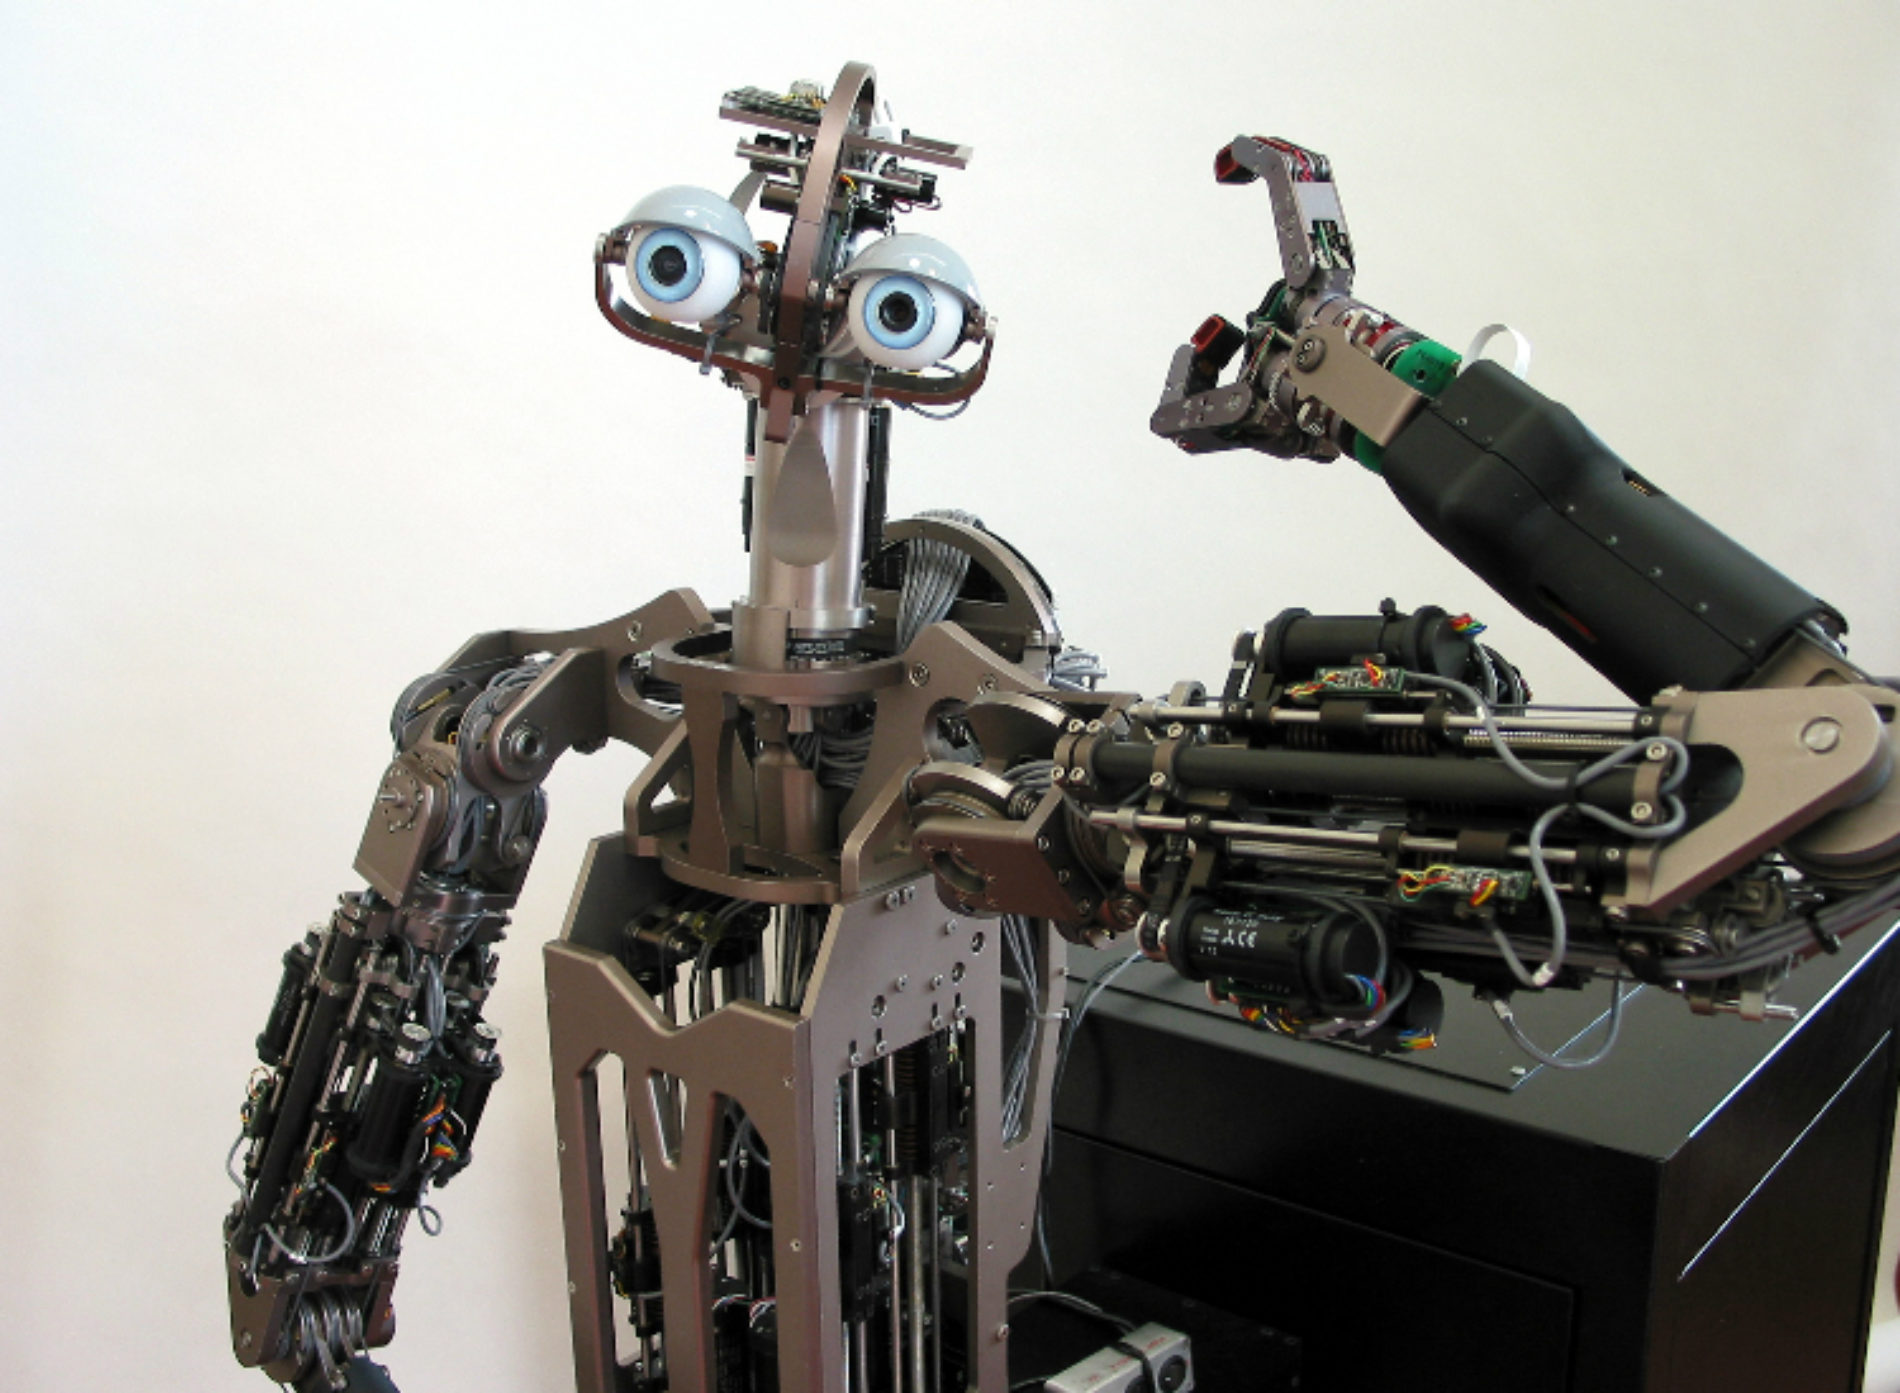
\includegraphics[width=0.6\linewidth]{tex/figs/domo-foto.jpg}
    \caption{Foto Robô Domo (Fonte: http://www.robotsvoice.com)}
    \label{fig:domorobot}
\end{figure}

Este projeto teve particular importância pois muitos dos conceitos explorados vieram a compor patentes e futuramente partes dos robôs Baxter e Meka, respectivamente das empresas Rethink Robotics e Meka Robótics. Da mesma equipe que desenvolveu o Domo surgiu a Meka Robótics a partir de Aaron Singer e Jeff Weber. E dos trabalhos de Pratt e Williason \cite{pratt1995series} surgiu a empresa Rethink Robotics fundada por Rodney Brooks, então professor do MIT em 1995.

% Baxter vs Meka
Embora com design completamente diferente, ambos robôs incorporam o uso atuadores série elásticos em cada uma das juntas como elemento de segurança. Desta forma qualquer pessoa pode manusear os braços de ambos robôs de maneira livre. No entanto este sistema também confere ao robô uma maior suscetibilidade a influência de outros estímulos externos como a ação da gravidade na dinâmica do robô tornado necessária o uso de soluções de controle complementares para garantir a precisão. \cite{nobody} Este problema é resolvido de forma diferente em cada uma das plataformas. No Baxter a compensação da gravidade é feita de forma completamente mecânica por uma série de molas \cite{nobody}, o que em parte explica seu maior tamanho. E no Meka esta é feita via software através do modelo dinâmico em conjunto da biblioteca KDL \cite{nobody}, conferindo um design mais compacto. 

% Robonauta -> Paradigmas atuais

\section{Definição do problema}

No Laboratório de Automação e Robótica ( LARA - UnB ) encontra-se disponível o braço robótico Meka A2 fornecido pela Meka Robotics. Daqui em diante será denominado apenas Meka. O Meka é um braço complacente antropomórfico composto por 7 juntas e uma garra desenvolvido para pesquisas na área de interação com pessoas. Cada uma das juntas possui um atuador série elástico composto de um motor sem escova e um redução mecânica por onda de deformação.

Em trabalhos anteriores foi observado um desempenho ineficiente nos controles cinemáticos implementados em contraste ao resultado observado em outras plataformas robóticas e em simulação. Tal arquitetura não encontra-se devidamente documentada e detalhada. Desta forma, neste trabalho, propõe-se realizar uma caracterização mais detalhada desta arquitetura de controle para compreender sua implicação no desempenho dos controles cinemáticos testados e propor melhorias que resultem em trajetórias mais precisas levando em conta as características próprias do sistema.

\section{Metodologia}

% Rever completamente
Este trabalho foi desenvolvido em três etapas: estudo sobre teoria clássica de controle de manipuladores, revisão e acompanhamento de trabalhos anteriores feitos no LARA utilizando o Meka e por fim a investigação e experimentação usando a plataforma. Esta investigação foi feita a partir da métodos científicos de análise e síntese do processo. Por meio da análise foram estudados cada um dos componentes utilizados tanto de hardware como software em seu detalhes. E contraponto foi alguns dos fenômenos foram sintetizados por meio de simulações visando ampliar a compreensão de quais fatores ocasionam ao Meka um desempenho inferior outros braços robóticos avaliados pelos trabalhos de Murilo \cite{nobody} e Marcos \cite{nobody}.

\subsection{Estudo controle de manipuladores}

Inicialmente foi feito um estudo sobre a teoria clássica do controle cinemático e dinâmico de manipuladores incluindo a representação por cadeia cinemática usando matrizes homogenias e a simplificação através da notação de Denavit-Hatemberg.

\subsection{Revisão trabalhos anteriores}

Inicialmente foi feito um estudo sobre os trabalho anteriores desenvolvidos na plataforma no Laboratório de Automação e Robótica ( LARA - UnB ) bem como estratégias clássicas no controle de robôs industriais. Alguns destes trabalhos puderam ser acompanhados ao longo da execução como o caso dos trabalhos desenvolvidos por Marcos Pereira e pelo Rafael Koji de modo a facilitar a transmissão do conhecimento relacionado as contribuições de cada um ao projeto bem como presenciar as dificuldades relacionadas ao controle do braço robótico.

\subsection{Investigação e experimentação a partir da plataforma}

Após o estudo preliminar foi adotado uma metodologia de investigação baseada em ciclos compostos por 3 etapas, descritas a seguir. Estas etapas são baseadas nos princípios de desenvolvimento ágil \ref{noref} e têm como objetivo acelerar e otimizar os esforços.

% TODO Colocar Referência

% Diagrama das etapas
\begin{enumerate}
    \item Análise e Formulação de Hipóteses
    \item Formulação de Testes para as Hipóteses
    \item Avaliação de Hipóteses ( Testes Experimentais e Estudo teórico )
\end{enumerate}

Cada ciclo possui duração variável de acordo com o nível de aprofundamento necessário para satisfazer os objetivos levantados para cada momento do projeto. O objetivo central é ao final de um ciclo é trazer algum aprimoramento quanto ao entendimento do sistema ou ainda quanto ao comportamento final na realização da tarefa.

No inicio de cada ciclo é feito um estudo do sistema através da modelagem do sistema e da definição de uma métrica para avaliar o comportamento. Então o comportamento do sistema real é comparado com o modelo adotado e as expectativas de comportamento. Os objetivos são traduzidos em uma métrica, compondo um conjunto de indicadores que permita avaliar se tarefa foi executada e como foi o processo de execução. A cada novo aspecto avaliado podem ser introduzidos novos indicadores em conjunto aos antigos ou modificados. 

Com base nisto são levantadas hipóteses quanto ao comportamento quanto ao fato de satisfazer ou não o modelo adotado e possíveis condutas para aprimorar os resultados dentro da métrica proposta. Para cada uma destas condutas é levantado um teste de verificação que pode incluir consulta bibliográfica, simulações a partir do modelo e experimentos com o Meka. Os resultados desta etapa são então levados para a etapa de observação e confrontados novamente e assim o ciclo se repete.

Resultados positivos são incorporados e resultados negativos avaliados quanto a possíveis correções. Tudo é registrado para permitir futuras avaliações. O resultado de cada dia foi feito um registro das atividades e todo material produzido foi colocado no GitHub \footnote{www.github.com/lara-unb/Meka} de forma a permitir o uso futuro na validação do comportamento após modificações futuras.

\section{Estrutura do Documento}

Este trabalho está dividido em 5 capítulos visando facilitar o entendimento. Estes estão organizados da seguinte forma:

\begin{itemize}
    \item \textit{Cap. \ref{ch:intro} Introdução} : Breve Apresentação e Histórico sobre Robótica Colaborativa.
    \item \textit{Cap. \ref{ch:teory-reference} Fundamentos} : Conceitos teóricos e tecnologias usadas no trabalho.
    \item \textit{Cap. \ref{ch:develop} Desenvolvimento} : Metodologia usada na investigação dos problemas e análise dos dados.
    \item \textit{Cap. \ref{ch:results} Resultados} : Dados obtidos ao longo do trabalho.
    \item \textit{Cap. \ref{ch:conclusoes} Conclusão} : Resultado final do trabalho e propostas de trabalhos futuros.
\end{itemize}


% Fundamentos
% - Teoria por trás do problema
% - Tecnologias por trás do problema
\chapter{Fundamentos Teóricos}\label{ch:teory-reference}

% Quote: Sobre o ombros de gigantes

% Resumo opcional. Comentar se não usar.
%\resumodocapitulo{Resumo opcional}

A primeira etapa de qualquer processo na engenharia é modelagem. A partir dela relacionamos todos conhecimentos relacionados a um sistema em busca de avaliar o comportamento através de uma descrição mais simplificada. Uma das principais formas é a modelagem matemática, em que é descrito as relações lógicas entre cada parte do sistema,. E assim podemos através de operações matemáticas analisar em profundidade bem como extrapolar o estudo para sistema com modelos parecidos.

O manipulador é modelado como uma série de barras ligadas entre si, cada qual aproximada como um corpo rígido. Assim o movimento completo do manipulador é descrito a partir do conjunto dos movimentos de cada uma das  um corpo rígido pode ser descrito de forma cinemática ou dinâmica. 

% o que é efetuador, junta ?

\section{Modelagem Cinemático}

Na abordagem cinemática estamos interessado apenas no movimento em si, independente das forças que o causaram. Desta forma são observados a posição, velocidade e aceleração de cada parte. Em um manipulador robótico, de forma geral, os movimentos são escolhidos em busca da resolução de uma tarefa pela localização de alguma ferramenta acoplada ao braço. Estas por sua vez são posicionadas no última junta por ser o ponto de maior alcance.

% O que é uma cadeia cinemática ?

Cada junta é controlada de maneira separada, assim para o controle da ponta é preciso converter o configuração das juntas somadas ao modelo geométrico das partes do braço para uma orientação e posição do efetuador no espaço em relação a base do manipulador.

% Cinemática


\subsection{Descrição DH}

Cada barra do braço, pode ser descrita a partir dos dois pontos em cada uma das extremidades. Por sua vez cada um dos pontos é definido por 6 parâmetros, 3 para a posição em relação aos eixos x,y e z e 3 para orientação a partir da rotação em relação a cada um dos eixos. Somando 12 parâmetros para cada barra. 

Como forma de reduzir a quantidade de parâmetros necessários para cada link é adotado uma convenção baseada em apenas 4 valores denominada parâmetros de Denavit-Hatemberg. Cada barra é descrita a partir de 2 valores de distância e dois ângulos. Esta redução leva em conta que as partes do braço estão sempre conectadas e por tanto a descrição a partir dos pontos nas extremidade traria sempre redundância nos valores. Assim é descrito a relação entre cada um dos pontos através das medidas da distância e orientação dos encaixes nas extremidades de cada barra.

% Ilustração DH

% Configuração de junta?
Estes parâmetros são definidos de tal forma que apenas um possui variação com o acionamento. Em juntas prismáticas este representa variação da distância enquanto em enquanto em juntas cilíndricas um do ângulos que variam. Quando ocorre mais 
O registro de posição atual de cada junta representa a configuração da junta. 

A partir da descrição é feito várias operações de mudança de base para relacionar a posição e orientação do efetuador em relação ao ponto da base. Para cada uma das juntas do braço é avaliado a variação da orientação e da posição em relação a extremidade da junta anterior. A partir da combinação destas operações em cadeia é possível determinar uma expressão relacionando a configuração de cada junta com a posição final

\subsection{Descrição Vetorial}

\subsection{Matrizes Homogenias}

\subsection{Quatérnions Duais}
\subsubsection{Números Complexos}
\subsubsection{Quatérnions}
\subsubsection{Números Duais}
\subsubsection{Representação por Quatérnions Duais}

A representação em quatérnions duais traz como vantagens: eliminar a singularidades, inexistência de ambiguidade de representação. Além de trazer uma representação mais compacta e portanto computacionalmente mais eficiente, uma vez que são utilizados 8 parâmetros ao invés de 12. % Citar paper IROS Bruno Adorno

São utilizados dois quatérnions, sendo um para a representação da posição e um quatérnion unitário para representação da orientação. 

\section{Controle}



% Definição de Controle

\subsection{Controle PID}

\subsection{Controle em Cascata}

% Desenvolvimento
\chapter{Desenvolvimento\label{ch:develop}}

\resumodocapitulo{Simple, clear purpose and principles give rise to complex, intelligent behavior. Complex rules and regulations give rise to simple and stupid behavior.(Hock Dee)}

\section{Desempenho de Sistemas Mecatrônicos}

Em trabalhos anteriores foram propostos e implementados vários controladores cinemáticos como forma de corrigir o efeito das pertubações devido a interação com uma agente externo e da ação da gravidade. No entanto o desempenho foi abaixo do apresentado pela código de demonstração do fabricante para o robô e pelos mesmos controladores no uso em outra plataforma explicitando a necessidade de um maior estudo da arquitetura do manipulador robótico Meka A2. Com base nisto foi feito uma análise do componentes do braço e a implementação dos sistemas de controle das juntas em software e hardware. Neste capítulo será descrito os métodos de investigação utilizados bem como experimentos efetuados.

Em \cite{marcosps2016} Marcos propôs diversas métricas e avaliar os controladores cinemáticos implementados. Enquanto foi possível um excelente detalhamento da desempenho de cada um dos controladores, foi descoberto limitações na interação com a plataforma. Neste trabalho será analisado o robô enquanto sistema observando as implicações dos componentes mecânicos, sistemas embarcados e sistemas de controle operando de forma conjunta. O objetivo é avaliar dentro do que já foi implementado os limites de desempenho permitidos pela plataforma para permitir um melhor desempenho em trabalhos futuros.

\begin{figure}[H]
    \centering
    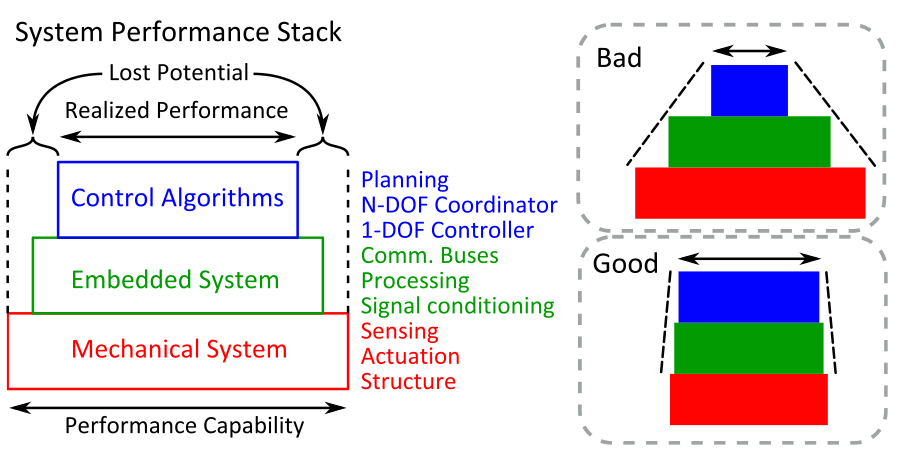
\includegraphics[width = 0.9\linewidth]{tex/figs/system_perfomance.png}
    \caption{Representação do Desempenho de um sistema \cite{paine2014high}}
    \label{fig:system_perfomance}
\end{figure}

Por se tratar de um sistema mecatrônico, naturalmente existem 3 camadas: Sistema Mecânico, Sistema Embarcado e Algorítimos de Controle conforme ilustrado na figura \ref{fig:system_perfomance} proposta por N. A. Paine em \cite{paine2014high} para o desenvolvimento de um sistema série elástico de alta performance. Para o Meka estas camadas estão implementados na seguinte forma:

\begin{itemize}
    \item Sistema Mecânico ( Atuadores Série Elásticos )
    \begin{itemize}
        \item Motores Brushless
        \item Harmonic Drive
    \end{itemize}
    \item Sistema Embarcado ( Atuadores Série Elásticos )
    \begin{itemize}
        \item Placa DSP para controle dos motores
        \item Hub EtherCAT
        \item Interface EtherCAT para o computador
        \item PC com Linux Ubuntu 12.04 e Kernel RTOS Xenomai
    \end{itemize}
    \item Algoritmos de Controle
    \begin{itemize}
        \item Controle de Torque (DSP)
        \item Controle de Posição com Compensação da Gravidade (PC)
        \item Interface ROS
        \item Controle Cinemático
        \item Gerador de Trajetória
    \end{itemize}
\end{itemize}

Como forma de alcançar um maior desempenho com o Meka foram avaliadas cada parte quanto a possíveis limitações e assim orientar trabalhos futuros no controle do robô.

% Comentar sobre desempenho de sistemas
% - Como alcançar o maior desempenho do sistema ( Custo exponencial 99.9 )
% - Não linearidades identificadas

% Avaliação Sistema Mecânico
% - Estudo SEA
% - Documentação
% Avaliação Sistema Embarcado?
% - Documentação EtherCAT, RTOS, PC
% - Tempo de Resposta da Comunicação
% Avaliação Controle
% - Ensaios Estabilidade em Malha Fechada
% - Ensaios em Degrau

% TODO Colocar nos resultados:
%No qual foi observado que aspectos particulares da plataforma não foram levados em conta como a operação em regiões não lineares do sistema devido a saturação da velocidade e torque dos motores, tempos longo de atraso de comunicação entre o computador.

% Reprodução Resultados Marcos

\section{Avaliação Preliminar}

Inicialmente foi feito um estudo a partir do código de demonstração do fabricante feito em Python para avaliar quais as possíveis forma de controlar o braço. Em que foi levantando todos os controladores implementados na biblioteca m3 e testados individualmente através da API em Python. Foram analisados os seguintes controladores disponíveis pelo M3:

\begin{itemize}
    \item Controle de Posição
    \item Controle de Posição com compensação da gravidade
    \item Controle de Torque
    \item Controle de Torque com compensação da gravidade
    \item Controle de Velocidade
\end{itemize}

%Nesta avaliação foi notado que alguns dos controladores da m3 não estavam disponíveis nas interfaces em C++. 

Para avaliar o comportamento em conjunto dos controladores cinemáticos apenas o controlador de posição com compensação da gravidade foi utilizado, uma vez que este que é usado pelo ROS.

\section{Estudo Controladores Cinemáticos}

Para definir um ponto de referência para os ensaios e testes foram avaliados os controladores implementados por Marcos Pereira. A partir da melhor configuração para cada um dos controladores foram feitos experimentos ajustando os parâmetros da velocidade de atuação e nível rigidez para avaliar a influência nos resultados. Os experimentos foram executados foram feitos com base em duas trajetórias pré-definidas: deslocamento em linha reta na vertical e o desenho de um quadrado a partir de dois deslocamentos na vertical e dois na horizontal.

Nos experimentos de deslocamento em linha reta foram avaliados o intervalo de tempo até robô começar a responder e o controle estabilizar para diferentes taxas de amostragem da trajetória. Enquanto nos experimentos com a trajetória de quadrado foram avaliadas a resposta do robô para diferentes valores de ajuste dos controladores de junta quanto aos parâmetros de velocidade e rigidez.

%\subsection{Avaliação tempo de amostragem}

O estudo dos tempos de atuação foi obtido repetindo o mesmo experimento para o deslocamento em linha reta na vertical em diferentes condições de velocidade e rigidez. Neste experimento foi estudado o tempo necessário para o atuador começar a se mover dado um comando bem o tempo necessário para o controle convergir.

% Resultados

%\subsection{Estudo Interação do controle de rigidez}

\section{Layout Experimentos}

Como forma de avaliar a resposta do sistema para controle dos ângulos de junta foi proposto um teste com o uso de um degrau de referência de entrada em malha fechada. Este experimento foi efetuado utilizando as interfaces da M3 definidas pela API em Python e pelo ROS. Para ambos casos os dados obtidos foram registrados em arquivo utilizando a ferramenta rosbag com auxílio do nó \textit{shm\_humanoid\_interface}.

% Comentar sobre como a informação é publicada nos tópicos
% Levantamento dos problemas

% Investigação de possíveis causas

\subsection{ROS}

Robotics Operating System (ROS) é um \textit{middleware} desenvolvido para a robótica. Desenvolver um robô é uma tarefa muito complexa para uma pessoa só ou mesmo um grupo de pesquisa, de modo que o ROS atua conectando diversos \textit{frameworks}, bibliotecas permitindo o uso de uma variedade de tipos de hardware e linguagens de programação \cite{quigley2009ros}. De igual forma atua conectando toda a comunidade de robótica em uma linguagem comum. Seu desenvolvimento começou em 2007 reunindo conceitos de diversos projetos de software aberto existentes até então e com o passar dos anos se tornou um padrão dentro da comunidade, contando com implementação para diversos robôs comerciais e inclusive uma versão completa voltada para a industria.

Como exemplo temos o módulo \textit{MovitIt} ( figura \ref{fig:movit-baxter} ) que reúne varias aplicações para facilitar o planejamento de trajetórias bem como a definição dos parâmetros de ajuste dos controladores com auxílio de métodos heurísticos através da biblioteca OMPL \cite{openMPL}.

\begin{figure}[H]
    \centering
    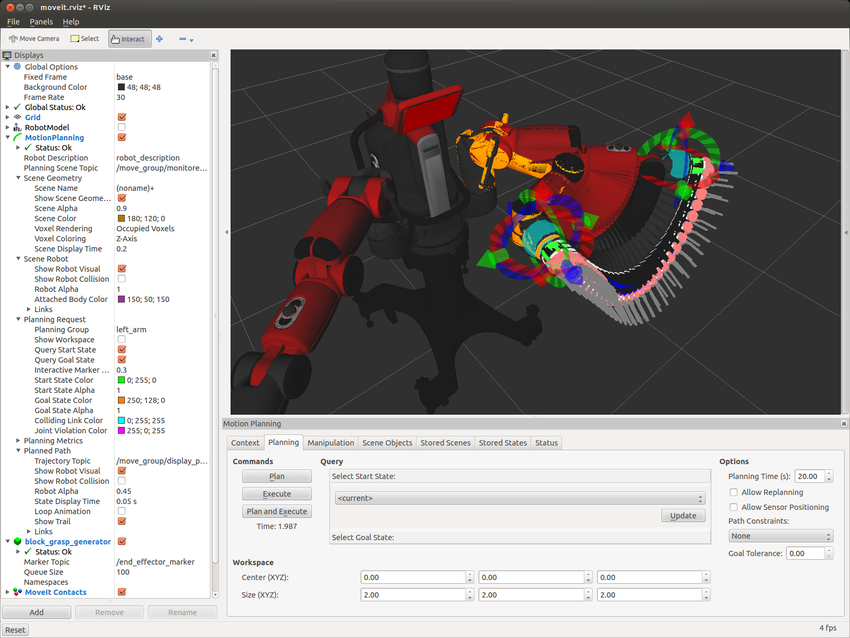
\includegraphics[width=0.7\linewidth]{tex/figs/movit-ros-baxter.png}
    \caption{Planejamento de Trajetória no Baxter com Auxílio do MoveIt \cite{coleman2014reducing}}
    \label{fig:movit-baxter}
\end{figure}

\subsection{shm\_humanoid\_interface}

Este é um nó do ROS disponibilizado pela Meka Robotics para a comunicação via ROS com o Meka. Representa uma das possíveis interfaces com a M3 através do acesso direto a memória compartilhada. em \ref{fig:mekaarch} são detalhados todas as possíveis interfaces. Através deste nó são gerados dois tópicos no ros: $/humanoid\_state$ e $/humanoid\_command$. A cada interação a informação atual do tópico $/hummanoid\_command$ é passada para a memória compartilhada e a leitura dos sensores é então escrita no tópico $/hummanoid\_state$. Na versão atual são somente interpretados os comando de posição das juntas através dos modos de controle com e sem compensação da gravidade.

\subsection{Rosbags}

Rosbags\footnote{\url{https://wiki.ros.org/rosbag}} é um utilitário do ROS para o registro dos eventos em cada tópico. A informação publicada nos tópicos é registrada em formato \textit{yaml} e permite que que posteriormente possa ser reproduzida em tópicos tal uma simulação. Desta forma dispensa a necessidade de manter o hardware conectado para analisar o comportamento do robô ao longo do tempo bem como permitir a análise de diferentes experimentos diretamente pelas ferramentas do ROS como o \textit{ros\_plot}. Ou ainda, permite conectar os resultados de um hardware real com uma simulação como forma de efetuar uma validação cruzada do comportamento real em comparação do comportamento simulado. Para tal basta executar o programa e indicar quais tópicos serão monitorados. Ao final da execução é registrado um arquivo com as informações com a extensão $.bag$. Internamente os dados são registrados em formato $.yaml$ o que permite a leitura direta.

Neste trabalho todos os experimentos foram registrados usando rosbag para permitir o uso futuro por outras pessoas. No entanto, como a representação da informação é um pouco verbosa gerando um arquivo grande, foi utilizado o programa $bag2csv$ para converter para o formato $.csv$ para facilitar o processamento. Em seguida o programa $sed$ para pequenos ajustes e a separação da leitura dos tópicos  $/humanoid\_state$ e $/humanoid\_command$ em diferentes arquivos. Este processo foi incorporado a um Makefile para permitir o processamento rápido de todos os arquivos $.bag$ utilizando o recurso de processamento paralelo da ferramenta \textit{GNU make}\footnote{\url{https://www.gnu.org/software/make/manual/html_node/Parallel.html}}.

\subsection{Python API}

A M3 possui uma interface através de uma API em Python que permite uma liberdade maior de controle uma vez que possui mais recursos já implementados. Além dos modos de controle por posição estão também disponíveis o controle direto por torque e por velocidade das juntas e o controle por PWM dos motores. Na M3 estão implementados um controlador para compensação da gravidade para o controle de torque e de posição a partir da biblioteca KDL com base no momento dinâmico do braço descrito no arquivo $m3ene/meka_doc/ma26/m3dynamatics\_right\_ma26.yml$. Este arquivo pode ser alterado para permitir o controle com um atuador com peso diferente, sem ter que alterar os parâmetros dos controladores.

% Explicação sobre funcionamento da biblioteca
% Diagrama: Comando/Estado -> Memória "bot" -> "proxy.step()"
% -> Problema Detectado no uso do ângulo em radianos por isto foi adotado o uso em graus

% Resultados
\chapter{Resultados\label{ch:results}}

% Simple, clear purpose and principles give rise to complex, intelligent behavior. Complex rules and regulations give rise to simple and stupid behavior. (Dee Hock)

% Resumo opcional. Comentar se não usar.
%\resumodocapitulo{Resumo opcional.}

% Resumo informações da arquitetura relevantes do ponto de vista de controle

%\section{Modelagem do Meka}
%\subsection{Estrutura controladores}

% \digraph[scale=0.5]{ab}{rankdir=LR; a->b;}

Para algum conhecimento se tornar cientifico é preciso a sistematização. Nesta capítulo serão apresentados os resultados qualitativos e numéricos do estudo feito em cima da plataforma.

\section{Estudo Arquitetura}

A primeira etapa foi de estudo do código e documentação em busca de identificar tecnologias e algoritmos envolvidos no controle do Meka. O intuito era identificar possíveis referências que ajudasse a guiar os experimentos a serem realizados e eventuais pontos críticos para o desempenho. Como a documentação oficial do Meka foi tirada fora do ar e apenas estão disponíveis as documentações geradas pela comunidade, foi feito um estudo para retirar possíveis pistas através do conhecimento deixado no código dentro do robô. Tal foi somente possível, pois por se tratar de uma plataforma voltada para pesquisa todo o código fonte estava disponível dentro do PC auxiliar.

% Arquitetura comunicação

No que foi 

\begin{figure}
    \centering
    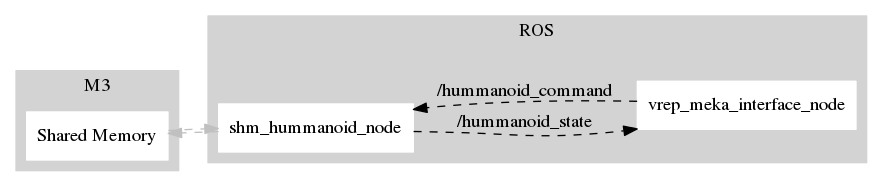
\includegraphics[width=1\linewidth]{figs/shm_arch}
    \caption{Caption}
    \label{fig:my_label}
\end{figure}


Todo o código relacionado ao controle do robô é disponibilizado pelo fabricante e compõe a biblioteca M3, implementada em Python e com interface em C++. A partir da análise do código foi possível observar alguns pontos importantes que contribuem para ineficiência dos controladores implementado anteriormente:

\begin{itemize}
    \item Apenas controle por posição de juntas está implementado em C++
    \item A taxa de atualização da memória compartilhada é de $100 Hz$
\end{itemize}

Dentro do programa de interface com o ROS foi possível observar alguns pontos importantes que contribuem para ineficiência dos controladores controladores de posição com e sem compensação da gravidade. Os valores de velocidade e torque informados para o controle são completamente ignorados. Além disto a taxa de envio da informação obtida pelo ROS para a memória compartilhada é de apenas $100Hz$ definidos \textit{hardcode}. Foi feito um teste para alterar este valor para $1KHz$ porém o robô ficou completamente instável. De movo que novos testes não foram repetidos para evitar danos ao robô.

Este valor é bem próximo das taxas de amostragem de $8 ms$ ($125 hz$) e $20 ms$ ($50 Hz$) dos controladores implementados em C++ obtidas para os melhores resultados em \cite{nobody} obtidos por Marco Pereira. Sendo estes valores definidos pelo tempo mínimo necessário para efetuar todos os cálculos relacionados ao controladores cinemáticos implementados usando quatérnions duais.

\section{Estudo Controladores Meka}

\subsection{API Python}

Para avaliar os controladores de junta de baixo nível foi utilizado a API em Python e a partir dai foram feitos vários teste a partir de comandos de posição para as juntas. A estrutura para envio dos comandos para o robô é diferente, de modo que alguns testes relacionados a comunicação também foram necessários. Estão estão disponíveis os seguintes controladores, ordenados do de mais alto nível para o de mais baixo nível:

\begin{itemize}
    \item Posição
    \item Velocidade
    \item Torque
    \item PWM
\end{itemize}

Todos estes estão disponíveis nos modos com e sem compensação da gravidade. 

\subsubsection{Avaliação do Atraso de Comunicação}

A comunicação com o robô é feita através de uma memória compartilhada. Assim, o primeiro experimento foi levantar o tempo gasto pela instrução \textit{proxy.step()} que atualiza esta memória pegando as medidas dos sensores e informando os comandos para os controladores. Este teste foi feito através avaliando o intervalo de tempo entre cada chamada após sucessivas interações tendo como resultado o valor médio de 16ms entre cada chamada indicando que a frequência máxima possível para um controlador implementado com base na API é de $f = 1/16ms = 62.5Hz$. Isto, obviamente, desconsiderando qualquer tempo extra gasto com as operações realizadas pelo próprio controlador.

\subsubsection{Avaliação do Acumulo do Erro}

Para verificar o acumulo do erro após sucessivas interações foi feito o teste de fechar a malha com braço na posição de repouso. Isto é, controle deveria ler os dados atuais do sensores e passar diretamente para o robô na expectativa de que o robô ficasse parado. No entanto foi observado que o braço começou a subir lentamente, indicando valores cada vez maiores para os ângulos medidos e uma distância cada vez maior da posição de origem.

Por outro ao ser enviado a mesma posição de referência suscetivamente, o braço desloca até o ponto desejado e permanece parado, mostrando que o controle para um referência em degrau é estável. O que viabilizou os testes de identificação a partir do uso de uma entrada em Degrau.

\subsubsection{Entrada em rampa}

Foram então feitos testes para um referência em rampa. Como se trata de um controle feito de maneira discreta, foram passados valores de ângulos em sequência incrementados por um valor contante e separados por um pequeno tempo de espera emulando uma entrada em rampa porém discretizada no tempo.

Para estudo da velocidade de resposta do controlador, o valor incrementado entre um ângulo e outro foi mantido enquanto o intervalo de tempo era ajustado. Neste experimento foi observado que para intervalos muito pequenos de tempo o robô não consegue acompanhar mantendo uma velocidade constante. Em tais casos a velocidade é mantida aproximadamente constante e com o acúmulo do erro ocorre saltos periódicos para compensar o atraso em relação a referência. Este fato decorre da interação entre o controlador de posição das juntas e o controlador de torque. O erro acumulado é corrigido com a passagem de um torque mais alto produzindo um salto na posição, seguido de uma leve oscilação para compensar o efeito da inercia.

% Repete testes ?

\subsubsection{Resposta ao Degrau}

Feito uma avaliação preliminar para o experimento de identificação da planta foi aplicado um degrau para cada uma das juntas individualmente com registro dos dados. Este teste foi definido a partir dos seguintes passos:

\begin{enumerate}
    \item Começa com a junta na posição $0$ graus
    \item Envia o comando para ir para posição $45$ graus
    \item Mantém a referência da posição em $45$ graus por $2s$
    \item Envia o comando para ir para posição $0$ graus
    \item Mantém a referência da posição em $0$ graus por $2s$
\end{enumerate}

Para a API em Python Estes passos foram executados 3 vezes para cada uma das juntas. O mesmo experimento foi efetuado a partir de um programa em C++ baseado no código elaborado em trabalhos anteriores. Para ambos casos a saída dos sensores foi registrada a partir do ROS a partir do programa rosbag e somente para os testes feitos em C++ foram também registradas os mensagens de controle. Uma vez que os comandos passados via API são enviados diretamente para o serializador de mensagens sem passar pelo ROS e portanto foram utilizados apenas para uma avaliação preliminar do comportamento dos controladores de junta.

% Qual foi a diferença dos dois para os mesmo parâmetros?
% Por que não foram avaliados outros ângulos?

\subsubsection{Controle de Posição sem Compensação da Gravidade}

O controle de posição sem o uso de compensação da gravidade foi avaliado em estudo e não foi possível atingir a posição desejada de 45 graus partido do zero em nenhuma das juntas. Na maioria dos caso o braço movia apenas 10 graus. O que explicita que toda a estratégia de compensação da gravidade é feita por software, diferente de outras plataformas como o Baxter em que esta é feita de forma mecânica.

\subsubsection{Controle de Velocidade}

Foi feito apenas um ensaio utilizando o controle de velocidade disponível na API em Python. No entanto ao ser definido velocidade zero a braço robótico ficou completamente rígido e passou a ignorar comandos para outros valores de referência de velocidade. O que demonstrou um esforço grande sendo feito pelo controle de torque e pelos motores. Somente quando foi alterado o modo de controle para posição que o braço voltou a mover normalmente. Para evitar qualquer dano a plataforma, não foram feitos outros testes neste modo de operação.

% Teria como controlar a velocidade diretamente ?

\subsubsection{Controle de Torque}

O controle de torque está disponível em dois modos: com e sem compensação da gravidade. Na estratégia sem compensação da gravidade, o valor de referência de torque é passado diretamente a controlador das juntas.

% Por que não foi avaliado o controle de torque?

\section{Estudo Controladores Cinemáticos}

\subsection{Resposta ao Degrau C++}

A velocidade máxima de cada junta pode ser ajusta para um valor entre $0$ e $1$, de igual forma a rigidez do braço gerada pelo controlador também pode ser ajustada entre $0$ e $1$. Valores maiores que 1 foram testados porém não houve mudança significativa em relação a comportamento com valor $1$.

Já no experimento feito de referência mostrado na \ref{fig:jointIdentification_exp2v100v50}, pode-se notar que existe um atraso de cerca de $20ms$ entre o comando e o recebimento do sinal de resposta do atuador no tópico. Também percebe-se um erro grande em regime permanente das juntas do pulso ($5$ e $6$). Percebe-se uma longa rampa indicando aonde o controle da posição passou a atuar como um controle tudo ou nada passando a velocidade máxima possível. Curiosamente, embora sejam motores distintos em cada uma das juntas com diferentes limites de velocidade a resposta do controlador é indica uma velocidade bem parecida de atuação nesta configuração.

\begin{figure}[H]
    \centering
    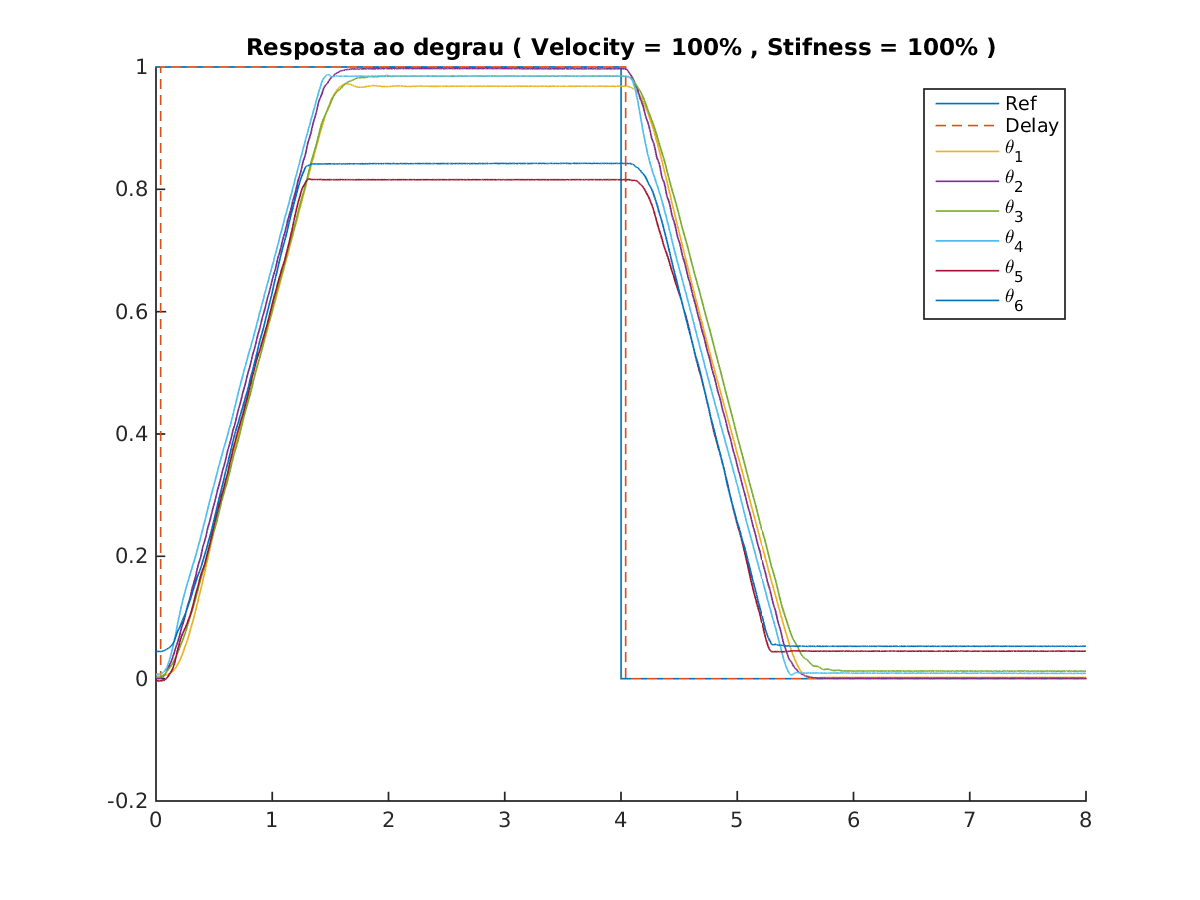
\includegraphics[width=0.6\linewidth]{tex/figs/jointIdentification_exp1v100v100.png}
    \caption{Resposta a um degrau de entrada com Velocidade = 1 e Rigidez = 1}
    \label{fig:jointIdentification_exp1v100v100}
\end{figure}

Pela figura \ref{fig:jointIdentification_exp2v100v50} observa-se que a variação da rigidez do controlador implica em um erro maior em regime permanente nas juntas. O controlador converge em um tempo próximo mas notadamente aumenta o erro das juntas do pulso. Este fato também é percebido no código de demonstração no ajuste da rigidez. Pois ao mudar o valor, mantida a mesma referência de posição o pulso desloca significativamente de posição.

\begin{figure}[H]
    \centering
    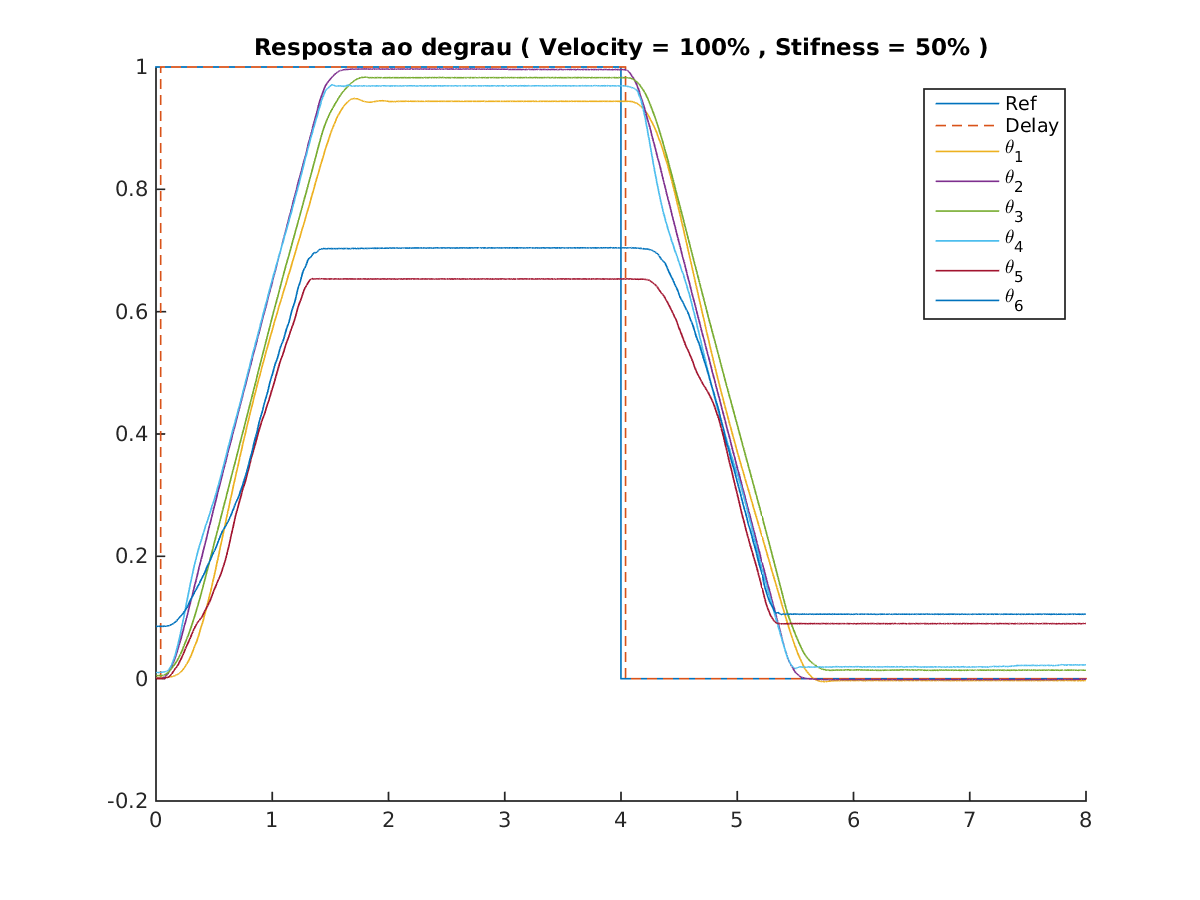
\includegraphics[width=0.6\linewidth]{tex/figs/jointIdentification_exp2v100v50.png}
    \caption{Resposta a um degrau de entrada com Velocidade = 1 e Rigidez = 0.5}
    \label{fig:jointIdentification_exp2v100v50}
\end{figure}

Como esperado, no terceiro experimento ao se alterar a velocidade para $70\%$ o tempo necessário para cada uma das juntas atingir a posição aumentou, tendo em vista a fase em que o controlador utiliza a velocidade máxima permitida, o erro em regime permanente para cada um permanece com pouca alteração. No entanto é percebido que a inclinação da curva durante as fase de controle entre o tempo $t=1s$ e $2s$ com a velocidade máxima muda de forma diferente para cada uma duas juntas. Estes dados encontram-se na figura \ref{fig:jointIdentification_exp3v70v100}.

\begin{figure}[H]
    \centering
    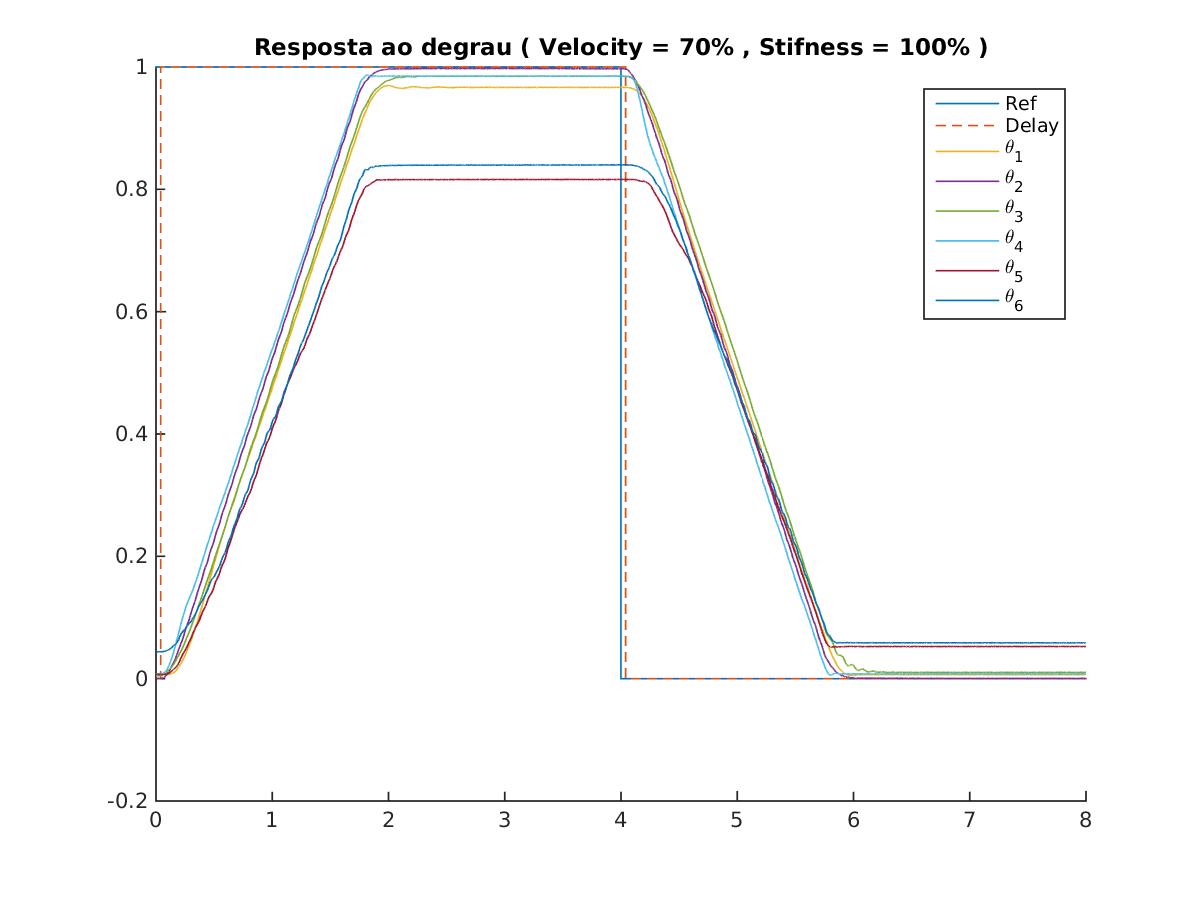
\includegraphics[width=0.6\linewidth]{tex/figs/jointIdentification_exp3v70v100.png}
    \caption{Resposta a um degrau de entrada com Velocidade = 0.7 e Rigidez = 1}
    \label{fig:jointIdentification_exp3v70v100}
\end{figure}

No 3 experimentos o atraso obtido foi próximo de $20ms$. Este valor é próximo dos valores de intervalo de tempo obtidos para os melhores resultados dos controladores implementados em \ref{nocite}. Notadamente, quando o controlador opera com frequências maiores, haverá o impacto do atraso da comunicação passa a ser mais significativo levando a instabilidade caso este não seja considerado no dinâmica implementada.


Tomando-se o diferença entre o valor passado de referência e o valor alcançado tempo foram obtidos os erro em regime permanente, registrados na tabela \ref{tab:jointIdentification_errortable}.

\begin{table}[H]
    \centering
    $$\begin{array}{cc|ccccccc}
         \hline
         V & S & \theta_0 & \theta_1 & \theta_2 & \theta_3 & \theta_4 & \theta_5 & \theta_6\\
         \hline
         -Inf & 0.031544 & 0.0025193 & 0.014824 & 0.014865 & 0.18436 & 0.15769\\
-Inf & 0.056071 & 0.0036188 & 0.017413 & 0.031003 & 0.34662 & 0.29566\\
-Inf & 0.033305 & 0.0026167 & 0.015199 & 0.014783 & 0.18398 & 0.16037\\
-Inf & 0.056453 & 0.0035564 & 0.017352 & 0.03028 & 0.32879 & 0.28538\\

         \hline
    \end{array}$$
    \caption{Error Percentual para diferentes valores de velocidade ($V$) e rigidez ($S$)}
    \label{tab:jointIdentification_errortable}
\end{table}

\begin{table}[H]
    \centering
    $$\begin{array}{cc|ccccccc}
         \hline
         V & S & \theta_0 & \theta_1 & \theta_2 & \theta_3 & \theta_4 & \theta_5 & \theta_6\\
         \hline
         0 & 1.0041 & 1.0001 & 1.0002 & 1.0025 & 1.0016 & 0\\
0 & 1.0049 & 1.0004 & 1.0008 & 1.0019 & 1.0007 & 0\\
0 & 1.003 & 1.0002 & 1.0004 & 1.0016 & 0 & 0\\
0 & 1.005 & 1.0004 & 1.0009 & 1.0026 & 0 & 0\\

         \hline
    \end{array}$$
    \caption{Percentual Overshot para diferentes valores de velocidade ($V$) e rigidez ($S$)}
    \label{tab:jointIdentification_overshottable}
\end{table}

\begin{table}[H]
    \centering
    $$\begin{array}{cc|ccccccc}
         \hline
         V & S & \theta_0 & \theta_1 & \theta_2 & \theta_3 & \theta_4 & \theta_5 & \theta_6\\
         \hline
         1.00 & 1.00 & 0.001841 & 0.96846 & 0.99748 & 0.98518 & 0.98513 & 0.81564 & 0.84231\\
1.00 & 0.50 & 0.003698 & 0.94393 & 0.99638 & 0.98259 & 0.969 & 0.65338 & 0.70434\\
0.70 & 1.00 & 0.0020654 & 0.9667 & 0.99738 & 0.9848 & 0.98522 & 0.81602 & 0.83963\\
1.00 & 0.50 & 0.0047216 & 0.94355 & 0.99644 & 0.98265 & 0.96972 & 0.67121 & 0.71462\\

         \hline
    \end{array}$$
    \caption{Valor em regime permanente para diferentes valores de velocidade ($V$) e rigidez ($S$)}
    \label{tab:jointIdentification_steadstatetable}
\end{table}

\subsection{Controladores Cinemáticos usando Quatérnions Duais}

% Experimento MoveUP

Os controladores de posição do efetuador foram avaliado a partir da estratégia de discretização dos pontos e frequência de amostragem. Para tal foi reduzido o número de ponto e trajetória foi simplificada para apenas um deslocamento em linha reta de 10cm na vertical. Para primeira análise foi utilizado os controladores implementados anteriormente e foram feitos os seguintes testes:

\begin{enumerate}
    \item Trajetória dividida em $100$ pontos, intervalo de $8 ms$
    \item Trajetória dividida em $100$ pontos, intervalo de $100 ms$
    \item Trajetória dividida em $1000$ pontos, intervalo de $8 ms$
\end{enumerate}

Foi observado que o robô leva um tempo até começar a mexer e um tempo até o controle estabilizar. De modo que está sempre atrasado em relação a referência. Para o período $8 ms$ foram necessárias $25$ interações até o robô começar a se mover, com o período de $100 ms$ o robô começo a se mover já na segunda interação sugerindo um atraso na comunicação de $200 ms$ entre o tempo que o comando é passado via ROS e o tempo que o robô executa o comando.

% Gráficos ?

% Saltos a cada 300 ms

\section{Estudo sobre não linearidades}

% Acrescentar simulação no simulink pControlSaturation
% - Comparativo da resposta para o mesmo ganho em um sistema de primeira ordem ( com delay e saturação )
% - Verificar necessidade de mudar a ordem e puxar a seção para antes

Uma vez que os modelos usados para o controle são lineares, a existência de comportamentos não lineares representam perturbações e podem gerar erros ou até instabilidade no controle caso não consideradas. Em razão disto uma atenção especial foi dada a este aspecto visando identificar a contribuição da perca de desempenho. A grande dificuldade é podem ocorrem em qualquer uma das partes do sistema de controle gerando um acumulo do efeito com o aumento da quantidade de camadas em cascata.

\subsection{Saturação do Atuador}

O efeito de saturação do atuador ocorre quando é solicitado uma ação de torque ou velocidade acima do que o atuador permite. Em diversos sistemas isto é limitado através de algum dispositivo de proteção evitando danificar o atuador. Do lado do controle, este é percebido como uma resposta mais lenta que o esperado para aquele determinado ganho em simulação podendo levar a instabilidade no controle do sistema real.

Como o controle da posição é feito em colaboração pela ação de cada uma das juntas, este problema é mascarado na métrica do erro de posição. Como a contribuição de cada junta em manipulador não cartesiano muda de acordo com a posição, o atraso devido a saturação pode fazer com que o robô tenha um erro maior para determinadas posições no decorrer da trajetória que outras. Outro efeito é a saturação de um motor levar a um uso maior dos outro motores na tentativa de compensar o erro acumulado.

São utilizados diferentes motores para cada uma das juntas, conferindo limitações especificas na atuação, em particular na velocidades máximas que cada junta pode atingir. Por conta disto, é percebido um maior uso das juntas com velocidade máxima maior para compensar o erro acumulado pela juntas com velocidade máxima menor, quando o controle começa solicitar uma velocidade maior que a permitida pelos outros motores.

Em particular no Meka, este fenômeno leva a um uso maior das juntas do ombro para corrigir orientação ao invés das juntas do pulso. Sendo um braço antropomórfico, o comportamento intuitivo esperado é a preferência das juntas mais próximas ao tronco para atuarem mais na posição enquanto as juntas próximos ao efetuador corrigirem a orientação. Isto é refletido na Jacobiana, para uma mesma variação de ângulo o mudança na posição e orientação é maior para as juntas do ombro que para as juntas do pulso.

% Fenômeno Harakiri: O cotovelo do meka vai se aproximando do tronco com o passar do tempo, o robô move bruscamente com pertubações na orientação a partir da posição de referência usada nos trabalhos do Koji e do Marcos

% Montar experimento Harakiri 2DOF
% Montar experimento Harakiri Meka em simulação no Matlab
% Montar experimento Harakiri Meka real
% Estudo do erro por junta ao invés de por posição -> Pontuar necessidade introduzir novas métricas

\subsection{Atraso da Comunicação}

Dado a existência de várias camadas entre o controle cinemático e o atuador de fato, existe um atraso na comunicação que influência na dinâmica do sistema. O controlador cinemático interagem com o ROS que por sua vez interage com uma memória compartilhada que é atualizada com um frequência de $1 KHz$. Para avalia o atraso foi feito a medida a partir do ensaio em degrau, entre o tempo de envio do comando de controle no tópico $/humanoid_control$ e o primeiro instante em que a posição da junta atinge um valor diferente de zero na leitura do valor correspondente no tópico $/humanoid_state$. Uma vez que existe um pouco de ruído na leitura da posição, foi considerado a valor de referência $\Delta\theta_0 = 0.1 rad = 5^\circ$.

% Resultados

\subsection{Controle Virtual de Rigidez}

% Comparar com primeiras implementações de SEA

Com base no controle do torque e o uso de sensores de posição pode se emular o comportamento de uma mola com rigidez variável através de um controlador. Esta estratégia é denominada mola virtual e permite conferir o controle de força com precisão sem a necessidade de ajustar fisicamente algum elemento elástico.

% Diagrama SEA Virtual

% Conclusão
\chapter{Conclusão} \label{ch:conclusoes}

\section{Perspectivas Futuras}

% Introdução 
% - Cobots
Neste trabalho foi apresentado um detalhamento maior da arquitetura de controle implementada no Meka permitindo conhecer os fundamentos das tecnologias envolvidas no desenvolvimento de manipuladores robóticos cooperativos bem como vivenciar os principais desafios em manter um manipulador robótico seguro e um desempenho razoável na execução de alguma tarefa. Foi buscado ir a origem inicial de cada problema, tanto do ponto de vista histórico como de cada componente utilizado. O redução no preço dos computadores, o uso de sistemas série elásticos para controle preciso de torque e bem como a disponibilidade de soluções open-source entre outras tecnologias permitiram que manipuladores robóticos pudessem alcançar mais pessoas. Soluções robóticas sempre estiveram no plano de tecnologias de alto padrão e distantes da realidade da maioria porém têm sido crescente os esforços na difusão.

% Fundamentação
% - Qualidade do HW
O Meka foi implementado com componentes de alto desempenho seguindo a filosofia do mercado na sua época de lançamento. Embora hoje, outras tecnologias estão sendo incorporadas ao projeto de robôs complacentes como o uso de sistemas freios, esta plataforma ainda representa uma ótima plataforma para o estudo de controladores dinâmicos bem como cada uma dos componentes envolvidos. Como exemplo, o uso de atuadores série elásticos, embora estejam implementados no Meka com motores e sistemas de transmissão de ponta, podem também ser incorporados em outros projetos como solução aos problemas de instabilidade do controle na interação com superfícies rígidas em aplicações para locomoção. Ou ainda em aplicação de forças na área de fisioterapia.

% Desenvolvimento
No que tange ao sistema de controle implementado, foi percebido que nos trabalhos anteriores foi alcançado o limite de desempenho dos controladores de baixo atuais do sistema M3. No entanto, dado que o sistema de controle é completamente open-source e possui um sistema embarcado capaz de uma desempenho maior ainda existe um enorme potencial que pode ser explorado para uso em trabalhos futuros. Uma vez que as soluções implementadas incorporam técnicas de filtragem e controle dinâmico que podem ser aprimoradas.

% Resultados
% - Juntas
Os controladores de posição de juntas foram ajustados para responderem de forma similar para todas as juntas. Embora esta seja uma estratégia que permite que a resposta controle seja similar e facilite a avaliação dos controladores cinemáticos, na prática o comportamento o comportamento de cada junta é bem diferente. Para um ganho de desempenho, pode ser explorado a possibilidade de controladores ajustados para respostas diferente para cada uma das juntas. Em conjunto com as características particulares da geometria do braço, um desempenho melhor pode ser atingido, por permitir as juntas do ombro operarem com uma resposta mais rápida.

A técnica atualmente implementada para compensação da gravidade usa apenas a posição das juntas para uma gerar um torque em feedforward a partir do modelo cinemático e dinâmico do robô. Outras técnicas podem ser utilizadas para que as velocidade final e o torque possam também ajustadas. Também foi notado que o acoplamento entre a posição e a orientação introduzido por quatérnions duais pode ser explorado a partir das características das juntas do robô, uma vez que a composição do ombro e do pulso podem atuar como dois guibal em oposição permitindo um estudo maior da dinâmica da rotação no movimento do efetuador.

% Trabalhos Futuros Controle + Metodologia
Para trabalhos futuros na plataforma é sugerido a identificação do modelo dos atuadores série elástico disponíveis na plataforma visando a implementação de um controle de juntas mais preciso. No intuito de apresentar a modelagem completa do braço, uma vez que esta não está disponível. Também é apresentado a possibilidade de estudo em controle multivariado a partir de espaço de estados para permitir explorar os efeitos das não linearidade em composição com o modelo cinemático do robô, gerando uma solução que controle ao mesmo a cinemática e dinâmica do movimento. Os conceitos implementados na plataforma podem também compor partes de outros projetos com explorado por outras universidades que passaram a produzir seus próprios atuadores, braços e plataformas robóticas.

%Com base nos resultados obtidos, observou-se o controle implementado em ROS está sendo executado com um frequência maior que a resposta das camadas inferiores subsequentes de controle. Este fator pode estar causando uma instabilidade no controle, uma vez que o erro acumulado durante o tempo que o robô permanece parado até o ocorrer a resposta é compensado com um esforço maior de controle, percebido nos registros dos experimentos como saltos periódicos na velocidade. Estes efeitos eram percebidos com maior nitidez no eixo vertical, uma vez que a maior perturbação ao sistema se dava pelo efeito da ação do campo gravitacional.

%Como proposta, serão efetuados ao longo do trabalho a continuidade do estudo da plataforma em conjunto com a identificação da planta completa. Por se tratar de um sistema complexo que envolve diversos sub-sistemas atuando em conjunto, este estudo será pautado as principais influências de cada componente no controle final da posição do efetuador.

%Também serão analisado um comparativo das estratégias de controle por velocidade e por posição a partir da descrição cinemática implementada em Quatérnions Duais. O controle por velocidade apresenta uma resposta mais rápida que os controles de velocidade por retirar a necessidade e esperar a posição final ser atingida e eliminaria a necessidade do passo de integração por parte de alguns dos controladores implementados. Ao passo que poderia permitir o uso direto de controladores mais baixos, uma vez que os motores Brushless possuem os controle de torque e velocidade que são convertidos em posição por meio da placa DSP.

%Ao final, o objetivo é trazer desempenho melhor em termos de precisão no controle do Meka e facilitar o uso deste no laboratório em projetos futuros por meio do aprofundamento na documentação e estudo iniciados em trabalhos anteriores. Em conjunto é apresentado um detalhamento das sistemas empregados para inspirar o uso em projetos futuros de sistemas robóticos desenvolvidos pelo laboratório, uma vez soluções similares baseadas em atuadores série elásticos estão presentes muitos projetos recentes.

% Bibliografia ------------------------------------------------------

\renewcommand{\bibname}{REFERÊNCIAS BIBLIOGRÁFICAS}
\addcontentsline{toc}{chapter}{REFERÊNCIAS BIBLIOGRÁFICAS}

\bibliographystyle{abnt-num}
\bibliography{relatorio}
\nocite{mmurilo-biorob}
\nocite{book:siciliano:2009}
\nocite{Adorno2011}
\nocite{figueredo:2013}
\nocite{book:spong:}
\nocite{edsinger2004domo}
%\nocite{pratt1995series} % Cited!
% Citar Livro
% https://new.abb.com/process-automation/process-automation-service/reference-pages/single-loop-control-methods

% Anexos -------------------------------------------------------------
\anexos
\makeatletter
% não retirar estes comandos
 \renewcommand{\@makechapterhead}[1]{%
   {\parindent \z@ \raggedleft \setfontarial\bfseries
     \LARGE \thechapter. \space\space
     \uppercase{#1}\par
     \vskip 40\p@ }}
\makeatother

% Anexo I: Descrição do CD
%\chapter{Descrição do conteúdo do CD}

\label{AnCD}

Descrever CD.


%\refstepcounter{noAnexo}

% Anexo II: Programas Utilizados
%\chapter{Programas utilizados}

Quais programas foram utilizados?

%\refstepcounter{noAnexo}

\end{document}
